\documentclass[titlepage=firstiscover, captions=tableheading, bibliography=totoc]{scrartcl}
\usepackage[autostyle=true,german=quotes]{csquotes}
\usepackage{scrhack}
\usepackage{caption}
\usepackage[aux]{rerunfilecheck}
\usepackage{subcaption}        
\usepackage{fontspec}
\usepackage[dvips]{graphicx}
\usepackage{floatflt,epsfig} 
    
\usepackage{polyglossia}
\setmainlanguage{german}

\usepackage[unicode]{hyperref}
\usepackage{bookmark}
\title{V27\\ Der Helium-Neon-Laser}
\author{
Miriam Simm\\
\texorpdfstring{\href{mailto:miriam.simm@tu-dortmund.de}{miriam.simm@tu-dortmund.de}\and}{,}
Katrin Bolsmann\\
\texorpdfstring{\href{mailto:katrin.bolsmann@tu-dortmund.de}{katrin.bolsmann@tu-dortmund.de}}{}
}
\date{Durchführung: 15.06.2020 \\ Abgabe: -.06.2020}
\usepackage{amsmath} 
\usepackage{amssymb} 
\usepackage{mathtools}
\usepackage[
    math-style=ISO,
    bold-style=ISO,
    sans-style=italic,
    nabla=upright,
    partial=upright,
]{unicode-math}
    
\setmathfont{Latin Modern Math}

\usepackage[
  locale=DE,
  separate-uncertainty=true, 
  per-mode=symbol-or-fraction,
]{siunitx}

\usepackage{multicol}
\setlength{\columnsep}{1pt} %space between columns 

\usepackage{booktabs}
\usepackage[x11names, table]{xcolor}
\usepackage{graphicx}
\usepackage{grffile}
\usepackage{xfrac}
\usepackage{xcolor}

\usepackage{float}
\floatplacement{figure}{h}
\floatplacement{table}{h}
\usepackage[
  section,
  below,
]{placeins}

\usepackage{expl3}
\usepackage{xparse}
\ExplSyntaxOn
\NewDocumentCommand \E {} {\symup{e}}
\ExplSyntaxOff

% Literaturverzeichnis
\usepackage[
  backend=biber,
]{biblatex}
% Quellendatenbank
\addbibresource{literatur.bib}

\usepackage[
  version=4,
  math-greek=default,
  text-greek=default,
]{mhchem}
 

\raggedcolumns

\begin{document}

\maketitle

\FloatBarrier
\begin{figure}[h]
\begin{minipage}[t]{0.59\textwidth}
\vspace{0pt}
\section{Einleitung und Zielsetzung}
In diesem Versuch soll der normale und der anomale Zeeman-Effekt untersucht werden. Dieses geschieht anhand der blauen und roten Spektrallinien einer Cadmium Lampe.

Der Effekt wurde 1896 erstmal von P. Zeeman (1865-1945) beobachtet und beschreibt die Aufspaltung und Polarisation der emittierten Spektralinien eines Atoms
unter Einfluss eines externen Magnetfeldes \cite{quelle03}. Dieses Phänomen wurde drei Jahre später von H. A. Lorentz (1853-1928) mit dem Einfluss des Magnetfeldes auf die
von den Drehimpulsen induzierten magnetischen Momente der Elektronenhülle begründet.
\end{minipage}
\hfill
\begin{minipage}[t]{0.4\textwidth}
\vspace{0pt}
\centering
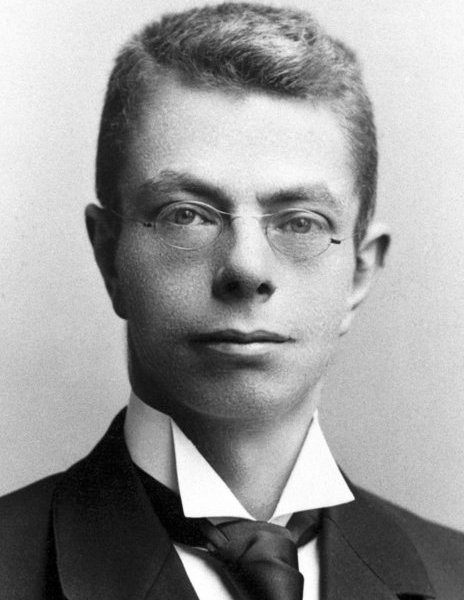
\includegraphics[height=5.0cm]{sexyTyp.png}
\caption{Pieter Zeeman (*25. Mai 1865; $\dagger$ 9. Oktober 1943) \cite{quelle03}.}
\label{fig:tfig1}
\end{minipage}
\end{figure}
\FloatBarrier

\section{Theorie}
\subsection{Das magnetische Moment}
Einem Hüllenelektron können zwei Arten von Drehimpulsen zugeordenet werden, der Bahndrehimpuls $\vec{l}$ und der Spin $\vec{s}$. Als Lösung der jeweiligen Eigenwertgleichung
ergeben sich die Beträge dieser Drehimpulse zu

\begin{align}
|\vec{l}| & = \sqrt{l(l+1)}\hbar \qquad \text{mit} \; l = 0,\, 1,\, 2,\, ... ,\, n-1 \label{eq:bahn}\\
|\vec{s}| & = \sqrt{s(s+1)}\hbar \qquad \text{mit} \; s = \frac{1}{2} \qquad . \label{eq:spin}
\end{align}

Da ein Elektron eine Ladung besitzt, induziert jedes Drehmoment auch ein magnetisches Moment. Allgemein ergibt sich zwischen einem Drehmoment $\vec{I}$ und dem durch diesen erzeugten magnetischen
Moment $\vec{\mu}_I$ der Zusammenhang

\begin{equation}
\vec{\mu}_I = - \mu_{\text{B}}g_I\frac{\vec{I}}{\hbar} \qquad . \label{eq:Moment}
\end{equation}

Hierbei ist $\mu_\text{B}$ das Bohrsche Magneton und $g_I$ der Landefaktor, welcher für den Bahndrehimpuls den Wert $g_L=1$ und für den Spin den Wert $g_S \approx 2$ besitzt.
Die Tatsache, dass das vom Spin $s=\frac{1}{2}$ erzeugte magnetische Moment etwa doppelt so groß ist wie das vom Bahndrehimpuls $l=1$ erzeugte, wird als \textit{magnetische Anomalie des Elektrons}
bezeichnet.

Mit den Beträgen für die Drehimpulse \eqref{eq:bahn} \eqref{eq:spin} lässt sich Gleichung \eqref{eq:Moment} explizit für Bahndrehimpuls und Spin angeben. 

\begin{align}
\vec{\mu}_l &= - \mu_{\text{B}}\sqrt{l(l+1)}\,\vec{l}_e \\
\vec{\mu}_s &= - g_S \mu_{\text{B}}\sqrt{s(s+1)}\,\vec{s}_e
\end{align}
Hierbei sind $\vec{s}_e$ und $\vec{l}_e$ jeweils die Einheitsvektoren in Richtung der Drehimpulse.
\\

In einem Atoms kommt es sowohl innerhalb eines Elektrons als auch zwischen den Einzelelektronen zu Wechselwirkungen zwischen den Drehimpulsen.
Je nachdem ob die Wechselwirkung innerhalb eines Elektrons oder die zwischen den einzelnen Elektronen überwiegt, lassen sich zwei Fälle unterscheiden.

\subsection*{LS-Kopplung}
Bei Atomen mit geringer Kernladungszahl ist die Wechselwirkung der Drehimpulse zwischen den Einzelelektronen so groß, dass sich die einzelnen Bahndrehimpulse und Spins der Elektronen zu je einem Gesamtdrehimpuls
zusammenfassen lassen
\begin{align}
\vec{L} &= \sum_i \vec{l}_i \qquad \text{mit}\; |\vec{L}| = \sqrt{L(L+1)}\hbar \\
\vec{S} &= \sum_i \vec{s}_i \qquad \text{mit}\; |\vec{S}| = \sqrt{S(S+1)}\hbar \qquad .
\end{align}

Den Gesamtdrehimpulsen für Spin und Bahndrehimpuls lässt sich wiederum je ein magnetisches Moment zuordnen, welche die Beträge
\begin{align}
\vec{\mu}_L &= \mu_{\text{B}}\sqrt{L(L+1)} \\
\vec{\mu}_L &= g_S \mu_{\text{B}}\sqrt{S(S+1)}
\end{align}
besitzen. Ist das Atom keinem zu großen Magnetfeld ausgesetzt, können Gesamtbahndrehimpuls und Gesamtspin zu einem Drehimpuls zusammengefasst werden
\begin{equation}
\vec{J}=\vec{L}+\vec{S} \qquad .
\end{equation}
Dies wird als \textit{LS-Kopplung} bezeichnet.

\subsection*{jj-Kopplung}
Bei Atomen mit einer hohen Kernladungszahl überwiegt die Wechselwirkung zwischen Spin und Bahndrehimpuls des Einzelelektrons. Somit kann lediglich der Gesamtdrehimpuls des Einzelelektrons
\begin{equation}
\vec{j}_i = \vec{l}_i + \vec{s}_i
\end{equation}
angegeben werden. Welcher sich zum Gesamtdrehimpuls des Atoms 
\begin{equation}
\vec{J} = \sum_i \vec{j}_i \label{eq:jj}
\end{equation}
addiert. Gleichung \eqref{eq:jj} wird als \textit{jj-Kopplung} bezeichnet.

\subsection{Aufspaltung der Energieniveaus im homogenen Magnetfeld}
Das zu dem Gesamtdrehimpuls $\vec{J}$ gehörende magnetische Moment $\vec{\mu}_J$ ist die Summe der magnetischen Momente von Spin und Bahndrehimpuls. Im Allgmeinen sind $\vec{\mu}_J$ und $\vec{J}$ nicht parallel, sodass sich $\vec{\mu}_J$ in eine zu $\vec{J}$ parallelen
und eine zu $\vec{J}$ senkrechte Komponente zerlegen lässt. Da das magnetische Moment eine Präzissionsbewegung um die Gesamtdrehimpulsachse durchführt, verschwindet der Erwartungswert der senkrechten Komponenten von $\vec{\mu}$.
Für den Betrag des magnetischen Moments ergibt sich mit dem Lande-Faktor $g_J$ des Atoms
\begin{align}
|\vec{\mu}_J| &= \mu_\text{B}g_J\sqrt{J(J+1)} \\
g_J &= \frac{3J(J+1)+S(S+1)-L(L+1)}{2J(J+1)} \qquad \label{eq:lande} .
\end{align}

In einem Magnetfeld unterliegt die Richtung des magnetischen Moments der sogenannten \textit{Richtungsquantelung}. Diese besagt, dass die zum Magnetfeld parallele Komponente von $\vec{\mu_J}$ immer ein ganzzahliges Vielfaches von $g_J\mu_{\text{B}}$ ist
\begin{equation}
\mu_{J,z}= -m g_J\mu_B \qquad .
\end{equation}
Wobei $\vec{B}=B\vec{e}_z$ angenommen wurde.
Da eine Vektorkomponente nicht größer als der Betrag des Vektors sein kann muss $|m|< J$ gelten. Somit ergeben sich für die sogennante \textit{Orientierungsquantenzahl} m, $2J+1$ mögliche Werte.
Für den Energiezuwachs eines Moments innerhalb eines Magnetfeldes gilt
\begin{equation}
E_\text{mag} = mg_J\mu_\text{B}
\end{equation}
und somit ergeben sich $2J+1$ äquidistante Energieniveaus, wie in Abbildung \ref{fig:tfig2} für J=2 dargestellt ist.

\begin{figure}
\centering
%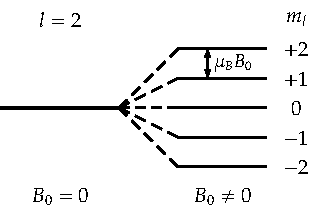
\includegraphics[height=5.0cm]{zeeman-effekt_2.pdf}
\caption{Die Aufspaltung der Energieniveaus in einem homogenen Magnetfeld für $J=2$. Hier entspricht $l=J$ und $m_l=m$ \cite{quelle04}.}
\label{fig:tfig2}
\end{figure}

Die Auspaltung betrifft auch angeregte Zustände, sodass beim Einschalten des Magnetfeldes auch eine Aufspaltung der emittierten Spektralinien beobachtet werden kann. Allerdings sind Übergänge nicht zwischen allen 
Energieniveaus möglich, sondern nur für solche für die $\Delta m \in \{-1, 0, 1\}$ gilt, wobei $\Delta m$ die Differenz der Orientierungsquantenzahlen der beiden Energieniveaus zwischen denen der Übergang stattfindet, ist.
Im Falle $\Delta m = 0$ ist die emittierte Strahlung parallel zum Magnetfeld linear polarisiert und wird $\pi$-Komponente genannt. Aufgrund der linearen Polarisationsrichtung können die Spektrallinien nur senkrecht zur Feldrichtung
beobachtet werden. Für $\Delta m = \pm 1$ ist die emittierte Strahlung zirkular um die Feldachse polarisiert und kann somit sowohl parallel als auch senkrecht zum Magnetfeld beobachtet werden. Diese wird als $\sigma$-Komponente bezeichnet.

\subsubsection*{Der normale Zeeman-Effekt}
Der normale Zeeman-Effekt beschreibt die Aufspaltung der Spektrallinien für Atome mit der Spinquantenzahl $S=0$. Somit ist der Gesamdrehimpuls gleich dem Gesamtbahndrehimpuls und für den Lande-Faktor ergibt sich $g_J=1$. Die Energieaufspaltung
\begin{equation}
    \label{eq:energie}
\Delta E = m \mu_\text{B}B
\end{equation}
ist also unabhängig von den Quantenzahlen $L$ und $J$. In Abbildung \ref{fig:tfig3} ist die Aufspaltung der Energieniveaus und die im vorherigen Abschnitt behandelten Übergänge zwischen diesen dargestellt.
\begin{figure}
\centering
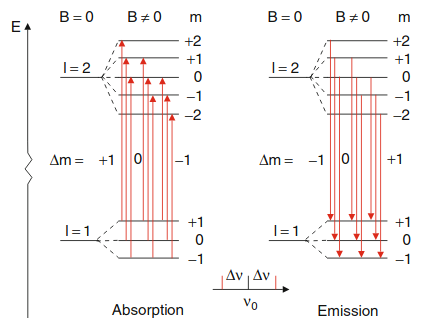
\includegraphics[height=8.0cm]{normalzeeman.png}
\caption{Der normale Zeeman-Effekt und Übergänge mit $\Delta m = \pm 1, 0$ \cite{quelle01}.}
\label{fig:tfig3}
\end{figure}

\subsubsection*{Der anomale Zeeman-Effekt}
Ist die Spinquantenzahl eines Atoms $S\neq 0$ wird die Aufspaltung der Energieniveaus in einem externen homogenen Magnetfeld als anomaler Zeeman-Effekt bezeichnet. Wie auch beim normalen Zeeman-Effekt sind nur Übergänge zwischen Energieniveaus
möglich für die $\Delta m \in \{-1, 0, 1\}$ gilt. Jedoch unterscheidet sich der anomale Zeeman-Effekt dadurch, dass die Verschiebung der Energieniveaus nicht mehr äquidistant ist. Somit ist die bei einem Übergang emittierte Strahlung abhängig von 
den Quantenzahlen $S, L$ und $J$ beider Niveaus und ist durch
\begin{equation}
E=(m_1 g(L_1, S_1, J_1)-m_2g(L_2, S_2, J_2))\mu_\text{B}B + E_0
\end{equation}
gegeben. Wobei es sich bei $E_0$ um das Energieniveau bei $B=0$ handelt. Die Lande-Faktoren können jeweils mit der Formel \eqref{eq:lande} bestimmt werden. In Abbildung \ref{fig:tfig4} ist das Termschema des anomalen Zeeman-Effekts in einem Na-Atom beispielhaft
dargestellt.
\begin{figure}
\centering
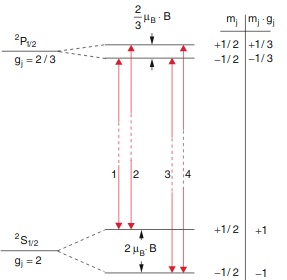
\includegraphics[height=8.0cm]{anomalerzeeman.png}
\caption{Der anomale Zeeman-Effekt am Beispiel eines Na-Atoms \cite{quelle01}.}
\label{fig:tfig4}
\end{figure}

\section{Versuchsaufbau}
Der Versuchsaufbau ist in Abbildung \ref{fig:tfig5} dargestellt.
\FloatBarrier
\begin{figure}
\centering
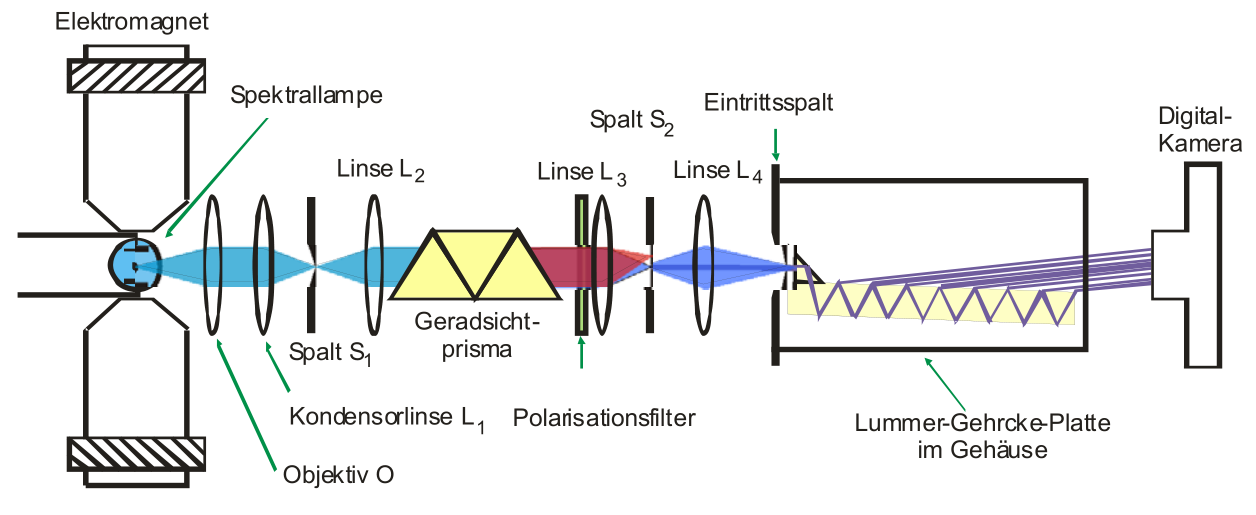
\includegraphics[width=\textwidth]{aufbau.png}
\caption{Experimenteller Aufbau zur Untersuchung des Zeeman-Effekts \cite{quelle02}.}
\label{fig:tfig5}
\end{figure}
\FloatBarrier
Zur Betrachtung des Zeemann-Effekts wurde eine Cadium-Lampe verwendet, welche sich zwischen den Polschuhen eines Elektromagneten befindet. 
Das Licht wird mittels eines Geradsichtprismas in die Spektralfarben aufgespaltet, sodass der normale
Zeeman-Effekt anhand der roten und der anomale Zeeman-Effekt anhand der blauen Spektrallinien untersucht werden kann. Mithilfe eines Polarisationsfilters können die linear polarisierten $\pi$-Komponenten
nach Bedarf herausgefiltert werden. Der Lichstrahl wird auf die Eintrittsfläche der Lummer-Gehrke Platte projiziert, durch diese wird ein Interferenzmuster erzeugt, 
welches mittels einer Digitalkamera aufgenommen werden kann. Im Folgenen soll noch einmal genauer auf die Lummer-Gehrke-Platte und dessen Funktionsweise eingegangen werden.

\subsection*{Die Lummer-Gehrke-Platte}
\FloatBarrier
\begin{figure}
\centering
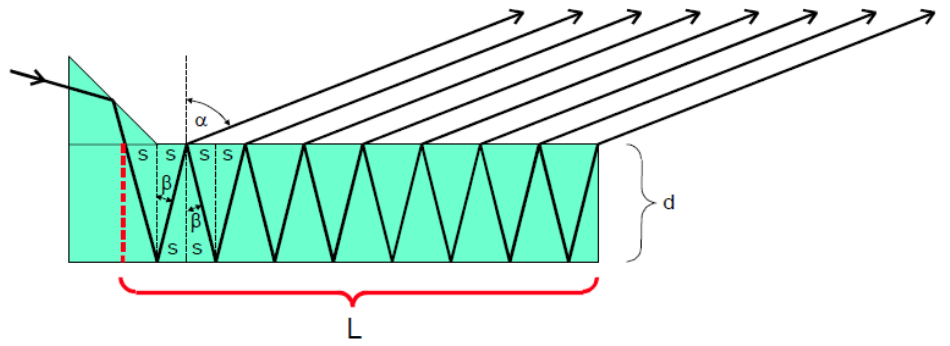
\includegraphics[width=0.8\textwidth]{dieguteGehrke.png}
\caption{Schematische Darstellung der Lummer-Gehrke-Platte und des Strahlenverlaufs \cite{quelle02}.}
\label{fig:tfig6}
\end{figure}
\FloatBarrier
Die Funktionsweise der Lummer-Gehrke-Platte ist schmematisch in Abbildung \ref{fig:tfig6} dargestellt. Das einfallende Licht wird innerhalb der Platte mehrmals totalreflektiert,
während bei jeder Totalreflektion ein Teil des Lichtstrahls transmittiert wird. Zwischen den austretenden Strahlenbündeln kommt es zur Interferenz. Kontruktive Interferenz tritt nur dann
auf, wenn die Bragg-Bedingung
\begin{equation}
2d \cos(\theta) = n \lambda
\end{equation}
erfüllt ist. Wobei $d$ die Dicke der Platte und $\lambda$ die Wellenlänge des einfallenden Lichtstrahls ist.
Bei monochromatischen Licht werden dementsprechend nur dann Interferenzstreifen erzeugt, wenn der Gangunterschied einem Vielfachen der Wellenlänge $\lambda$ entspricht. Da der Zeeman-Effekt zu einer 
Änderung der Wellenlänge um $\delta \lambda$ führt, ist eine Verschiebung der Interferenzstreifen um $\delta s$ zu beobachten.

Damit es zu keiner Überlagerung der Interfernzstreifen kommt, darf die Wellenlängendifferenz maximal
\begin{equation}
\Delta \lambda_D = \frac{\lambda ^2}{2d}\sqrt{\frac{1}{n^2-1}}
\end{equation}
betragen. Das Auflösungsvermögen der Lummer-Gehrke-Platte ist demnach gegeben durch
\begin{equation}
A = \frac{\lambda}{\Delta \lambda} = \frac{L}{\lambda}(n^2-1) \quad  .
\end{equation}
Hierbei ist $L$ die Länge und $n$ der Brechungsindes der Lummer-Gehrke-Platte.


\section{Durchführung des Versuchs}
Zu Beginn des Versuchs wird zunächste das Magnetfeld des Elektromagneten mit einer Hall-Sonde vermessen. Dazu wird der Strom zwischen $0\,\si{\A}-5\,\si{\A}$ variiert und die Magnetfeldstärke im Bereich der
Cd-Lampe notiert.
Anschließend wird die Apparatur so justiert, dass ein roter Lichstrahl mit möglichst hoher Intensität auf das Eintritssfenster der Lummer-Gehrke-Platte trifft und das Interfernzmuster auf der Digitalkamera sichtbar ist.
Es wird je eine Aufnahme mit und ohne Magnetfeld für beide Einstellungen des Polarisationsfilters gemacht, wobei einmal die zum Magnetfeld linear polarisierten Lichtanteile herausgefilert werden, sodass nur die $\sigma-$Komponenten
im Energiespektrum sichtbar sind.
Anschließend wird die Apparatur erneut justiert, sodass nun ein blauer Lichtstrahl auf die Lummer-Gehrke Platte trifft und die Prozedur wiederholt.

\section{Auswertung}
\subsection{Magnetfeldmessung}
Die gemessenen Werte der Magnetfeldstärke sind in Tabelle \ref{tab:atab1} dargestellt.
\FloatBarrier
\begin{table}[h]
    \centering
    \caption{Messwerte der Magnetfeldstärke in Abhängigkeit von der Stromstärke.}
    \begin{minipage}{0.45\textwidth}
        \centering
        \label{tab:atab1}
        \begin{tabular}{c c}
            \toprule
            {$I / A$} & {$B / \text{mT}$} \\
            \midrule
            0.5 & 46    \\ 
            1   & 92    \\
            1.5 & 137.5 \\
            2   & 183.1 \\
            2.5 & 223.0 \\
            3   & 268.7 \\
            3.5 & 306.8 \\
            4   & 345.0 \\
            4.5 & 377.3 \\
            5   & 408.9 \\
            \bottomrule
        \end{tabular}
    \end{minipage} \hfill%
    \begin{minipage}{0.45\textwidth}
        \centering
        \begin{tabular}{c c}
            \toprule
            {$I / A$} & {$B / \text{mT}$} \\
            \midrule
            5   & 414.5 \\
            4.5 & 388.4 \\
            4   & 354.9 \\
            3.5 & 316.7 \\
            3   & 277.5 \\
            2.5 & 230.8 \\
            2   & 189.8 \\
            1.5 & 144.2 \\
            1   & 95.9  \\
            0.5 & 51.2  \\
            \bottomrule
        \end{tabular}
    \end{minipage}
\end{table}
\FloatBarrier
\noindent
In Abbildung \ref{fig:afig1} sind die Werte grafisch dargestellt. Mit dem Paket $\texttt{SciPy.optimize.curve\_fit}$ wird außerdem 
eine Ausgleichsrechnung durchgeführt, wobei als Funktion ein Polynom dritten Grades verwendet wird
\begin{equation*}
    f \left(x\right) = a x^3 +b x^2 +c x +d \,
\end{equation*}
\FloatBarrier
\begin{figure}
    \centering
    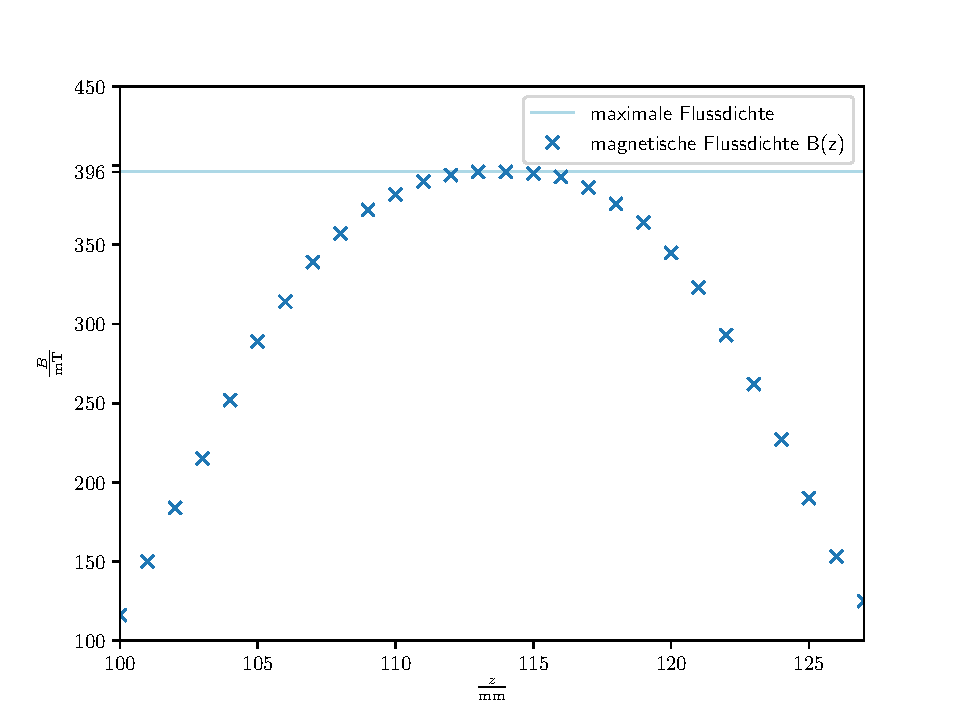
\includegraphics[width=0.8\textwidth]{magnetfeld.pdf}
    \caption{Messwerte der Magentfeldstärke in Abhängigkeit von der angelegten Stromstäke und Ausgleichskurve.}
    \label{fig:afig1}
\end{figure}
\FloatBarrier
\subsection{Rote Spektrallinie}
Mit der roten Spektrallinie wird der normale Zeeman-Effekt untersucht, weswegen nur die $\sigma$-Komponente betrachtet wird.
Die Aufnahmen bei $B = 0$ (oberes Bild) und $B \neq 0$ (unteres Bild) sind in Abbildung \ref{fig:afig2} dargestellt.
\FloatBarrier
\begin{figure}
    \centering
    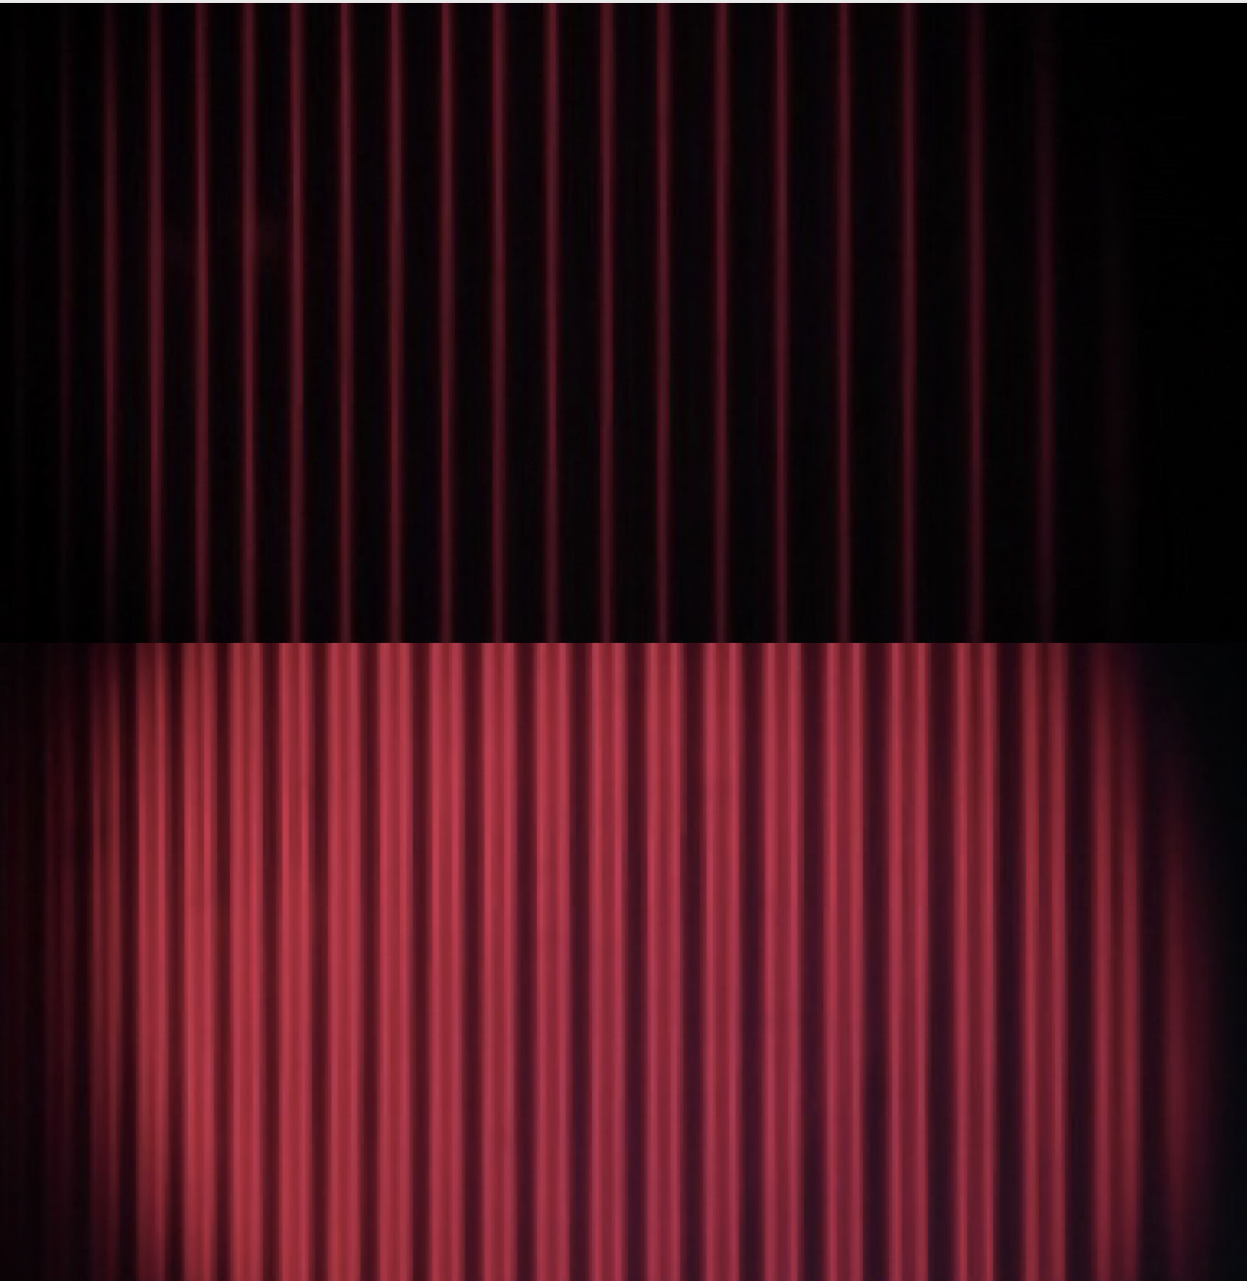
\includegraphics[width=0.8\textwidth]{rot.jpg}
    \caption{Aufnahmen mit rotem Licht bei ein- und ausgeschaltetem Magnetfeld.}
    \label{fig:afig2}
\end{figure}
\FloatBarrier
Zur Berechnung der Aufspaltung $\delta \lambda$ wird in der Aufnahme mit ausgeschaltetem Magentfeld \ref{fig:afig2} der 
Abstand der Spektrallinien $\Delta s$ bestimmt. Die Verschiebung $\delta s$ wird in der Aufnahme mit eingeschaltetem 
Magentfeld mit Magentfeldstärke $B = 421.3 \,\si{\milli\tesla}$ vermessen. Die Messung erfolgt in Pixeln (px).
Die Aufspaltung $\delta \lambda$ berechnet 
sich dann durch
\begin{equation}
    \label{eq:Auswertung}
    \delta \lambda = \frac{1}{2} \frac{\delta s}{\Delta s} \Delta \lambda_D \,
\end{equation}
wobei der Wert für $\lambda_D$ aus Tabelle \ref{tab:atab0} entnommen wird. 
Diese gemessenen Werte für $\delta s$ und $\Delta s$ sowie jeweils der berechnete Wert für $\delta \lambda$ sind in Tabelle \ref{tab:tab2} dargestellt.
\FloatBarrier
\begin{table}[h]
    \centering
    \caption{Messwerte der Abstände der Speltrallinien $\Delta s$ und der Verschiebung $\delta s$ sowie berechnete Auspaltung $\delta \lambda$.}
    \label{tab:atab2}
    \begin{tabular}{c c c}
        \toprule
        {$\Delta s / \text{px}$} & {$\delta s / \text{px}$} & {$\delta \lambda / \si{\meter}^{-11}$}\\
        \midrule
        15 & 5 & 0.8152 \\ 
        14 & 5 & 0.8734 \\
        15 & 6 & 0.9782 \\
        14 & 6 & 1.0481 \\
        16 & 6 & 0.9171 \\
        15 & 6 & 0.9782 \\
        16 & 6 & 0.9171 \\ 
        16 & 6 & 0.9171 \\
        17 & 6 & 0.8631 \\ 
        17 & 7 & 1.0070 \\ 
        17 & 7 & 1.0070 \\
        18 & 7 & 0.9510 \\
        19 & 7 & 0.9010 \\
        19 & 8 & 1.0297 \\
        20 & 8 & 0.9782 \\
        21 & 8 & 0.9316 \\
        21 & 8 & 0.9316 \\
        23 & 9 & 0.9569 \\
        \bottomrule
    \end{tabular}
\end{table}
\FloatBarrier
\noindent
Es wird nun mit dem $\texttt{Python}$-Paket $\texttt{NumPy}$ der Mittelwert aus allen
berechneten Werten für $\delta \lambda$ bestimmt. Der Fehler berechent sich hierbei nach Gauß'scher Fehlerfortpflanzung,
die ebenfalls mit dem Paket $\texttt{NumPy}$ durchgeführt wird. Es ergibt sich der Wert
\begin{equation*}
    \delta \lambda = \SI{0.9445(0143)e-11}{\meter}
\end{equation*}
Zur Berechnung des Landé-Faktors $g$ muss außerdem die Energiedifferenz $\Delta E$ bestimmt werden, wozu die Energie
\begin{equation*}
    E = \frac{\text{hc}}{\lambda}
\end{equation*} 
um kleine Änderungen der Wellenlänge $\Delta \lambda$ in erster Ordnung entwickelt wird. Es ergibt sich
\begin{equation*}
    \Delta E = \frac{\text{h c}}{\lambda^2} \Delta \lambda
\end{equation*}
Mit Gleichung \eqref{eq:energie} folgt dann für den Landé-Faktor die Formel 
\begin{equation} 
    \label{eq:landee}
    g = \frac{\text{h c}}{\lambda^2 B \mu_B} \Delta \lambda
\end{equation}
mit der sich für den Landé-Faktor der Wert
\begin{equation*}
    g = 1.159\pm 0.018
\end{equation*}
ergibt.

\subsection{Blaue Spektrallinie}
Die Vorgehensweise bei der Untersuchung der blauen Spektrallinie erfolgt analog, jedoch wird nun der anomale Zeeman-Effekt
untersucht, weswegen sowohl die $\sigma$- als auch die $\pi$-Linie betrachtet wird. 
Die Aufnahmen bei $B = 0$ (oberes Bild) und $B \neq 0$ (unteres Bild) sind in Abbildung \ref{fig:afig3} dargestellt.
\FloatBarrier
\begin{figure}
    \centering
    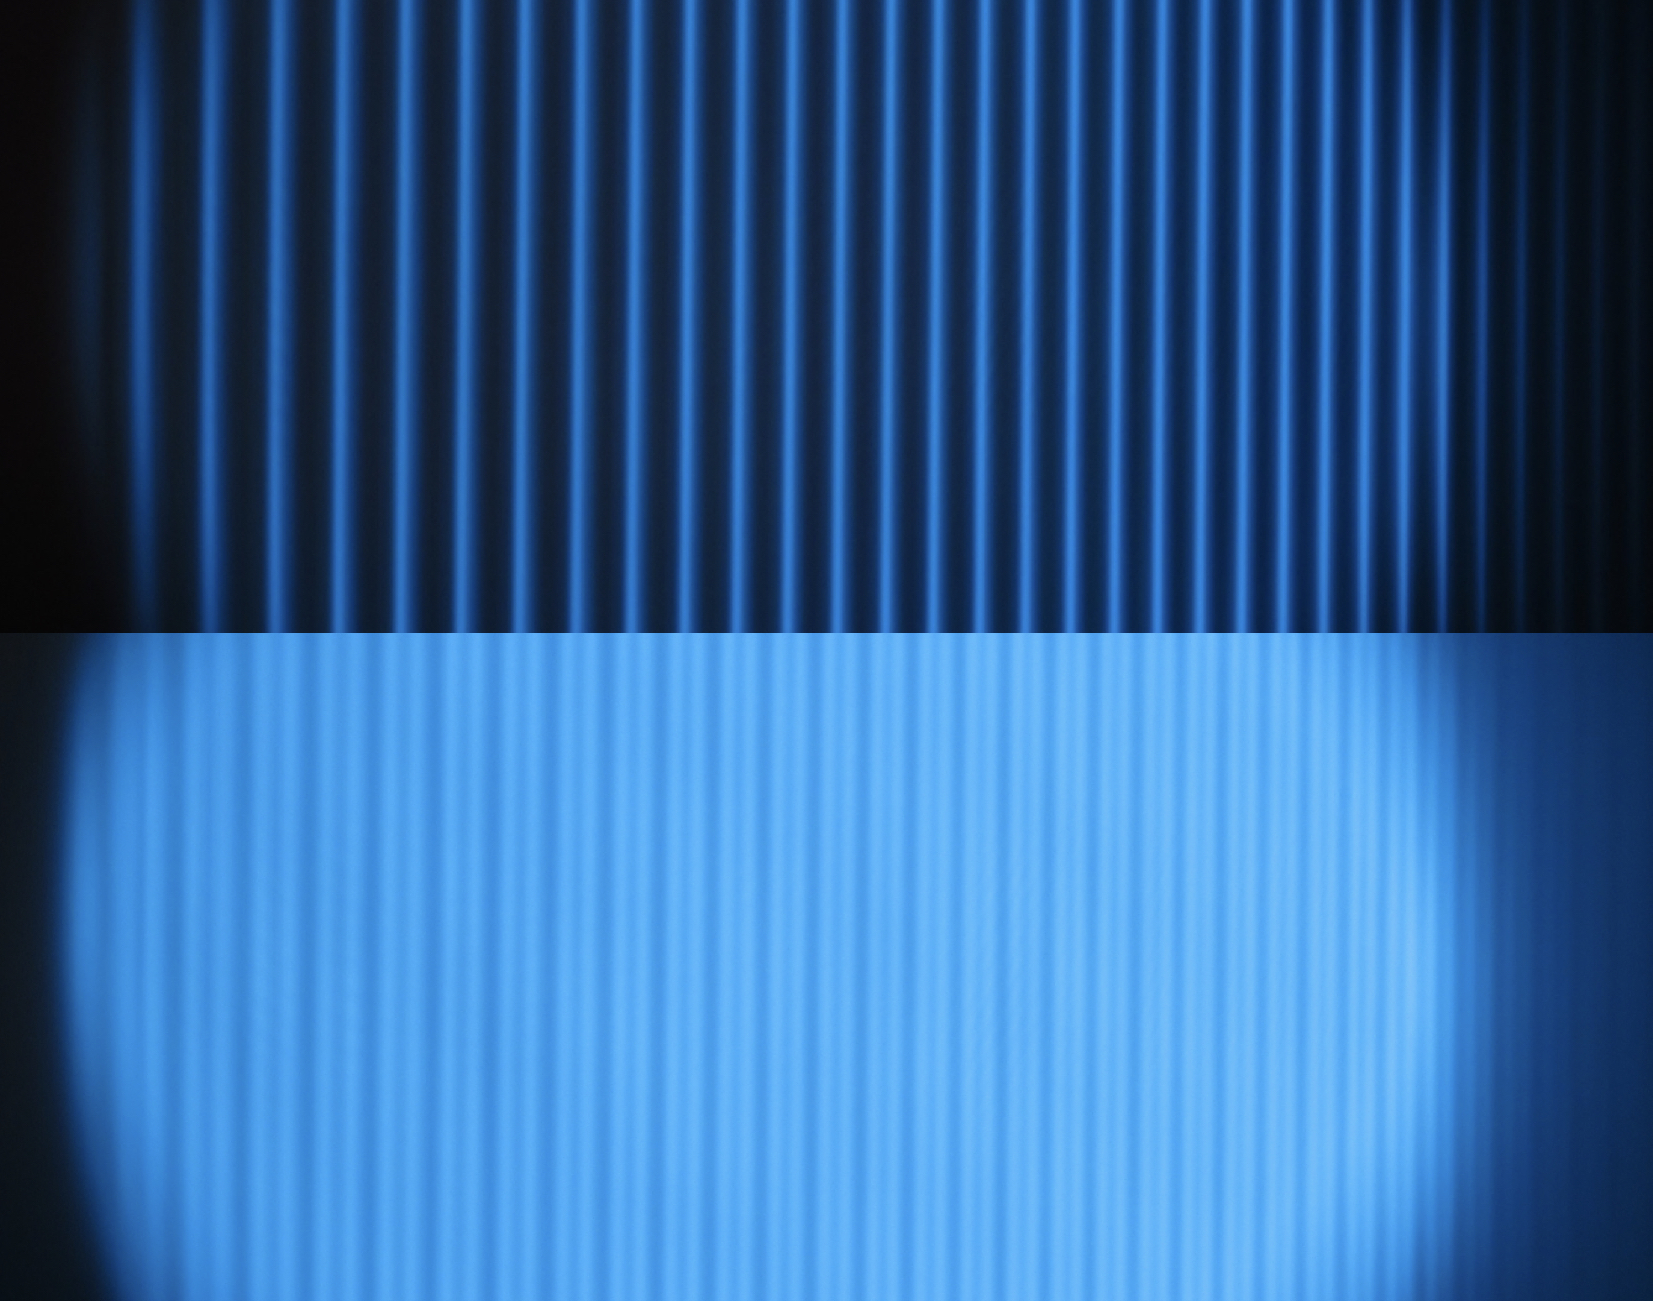
\includegraphics[width=0.8\textwidth]{pi.jpg}
    \caption{Aufnahmen der $\pi$-Linie mit blauem Licht bei ein- und ausgeschaltetem Magnetfeld.}
    \label{fig:afig3}
\end{figure}
\FloatBarrier
\subsubsection*{$\pi$-Linie}
Die $\pi$-Linie wird bei einem Magnetfeld von $B = 1009 \, \si{\milli\tesla}$ vermessen.
Die gemessenen Werte für 
$\delta s$ und $\Delta s$ sowie jeweils der berechnete Wert für $\delta \lambda$ sind in Tabelle \ref{tab:atab3} dargestellt.
\FloatBarrier
\begin{table}[h]
    \centering
    \caption{Messwerte der Abstände der Speltrallinien $\Delta s$ und der Verschiebung $\delta s$ sowie berechnete Auspaltung $\delta \lambda$ für die $\pi$-Linie.}
    \label{tab:atab3}
    \begin{tabular}{c c c}
        \toprule
        {$\Delta s / \text{px}$} & {$\delta s / \text{px}$} & {$\delta \lambda / \si{\meter}^{-11}$}\\
        \midrule
        116 & 74 & 0.8596 \\
        114 & 64 & 0.7565 \\
        111 & 58 & 0.7041 \\
        107 & 56 & 0.7052 \\
        104 & 51 & 0.6608 \\
        99  & 51 & 0.6942 \\
        97  & 48 & 0.6668 \\
        94  & 48 & 0.6881 \\
        92  & 49 & 0.7177 \\
        90  & 48 & 0.7187 \\
        87  & 50 & 0.7744 \\
        86  & 48 & 0.7521 \\
        83  & 49 & 0.7955 \\
        82  & 48 & 0.7888 \\
        81  & 46 & 0.7652 \\
        79  & 45 & 0.7676 \\
        76  & 44 & 0.7801 \\
        76  & 43 & 0.7624 \\
        75  & 42 & 0.7546 \\
        74  & 41 & 0.7466 \\
        71  & 42 & 0.7971 \\
        70  & 40 & 0.7700 \\
        70  & 38 & 0.7315 \\
        69  & 37 & 0.7226 \\
        66  & 39 & 0.7963 \\
        68  & 40 & 0.7926 \\
        \bottomrule
    \end{tabular}
\end{table}
\FloatBarrier
\noindent
Als Mittelwert ergibt sich
\begin{equation*}
    \delta \lambda = \SI{0.7488(0091)e-11}{\meter} \, .
\end{equation*}
Mit der obigen Formel \eqref{eq:landee} ergibt sich für den Landé-Faktor
\begin{equation*}
    g = 0.680 \pm 0.008 \, .
\end{equation*}

\subsubsection*{$\sigma$-Linie}
Aus den Aufnahmen in \ref{fig:afig4} für $B = 0$ (oberes Bild) und $B \neq 0$ (unteres Bild)
\FloatBarrier
\begin{figure}
    \centering
    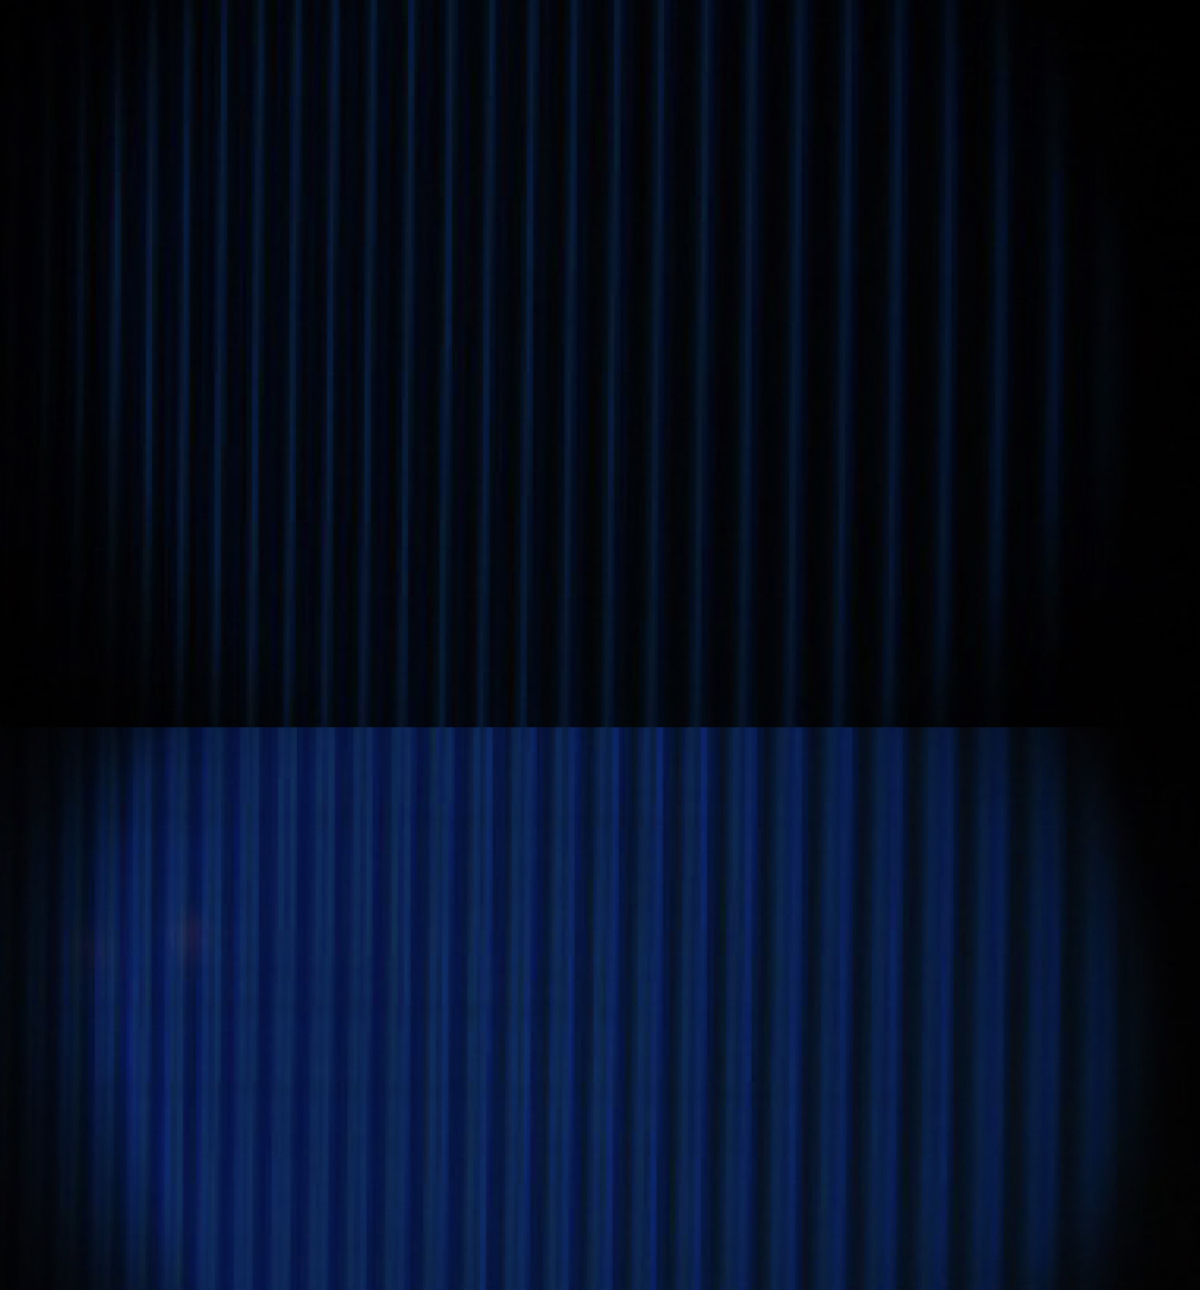
\includegraphics[width=0.8\textwidth]{sigma.jpg}
    \caption{Aufnahmen der $\sigma$-Linie mit blauem Licht bei ein- und ausgeschaltetem Magnetfeld.}
    \label{fig:afig4}
\end{figure}
\FloatBarrier
Die für die $\sigma$-Linie bei $B = 306.8 \, \si{\milli\tesla}$ bestimmten Werte sind in Tabelle \ref{tab:atab4} dergestellt.
\FloatBarrier
\begin{table}[h]
    \centering
    \caption{Messwerte der Abstände der Speltrallinien $\Delta s$ und der Verschiebung $\delta s$ sowie berechnete Auspaltung $\delta \lambda$ für die $\sigma$-Linie.}
    \label{tab:atab4}
    \begin{tabular}{c c c}
        \toprule
        {$\Delta s / \text{px}$} & {$\delta s / \text{px}$} & {$\delta \lambda / \si{\meter}^{-11}$}\\
        \midrule
        11 & 6  & 0.7350 \\
        11 & 6  & 0.7350 \\
        11 & 6  & 0.7350 \\
        12 & 6  & 0.6738 \\
        12 & 6  & 0.6738 \\
        12 & 6  & 0.6738 \\
        12 & 6  & 0.6738 \\
        12 & 6  & 0.6738 \\
        13 & 6  & 0.6219 \\
        13 & 7  & 0.7256 \\
        13 & 7  & 0.7256 \\
        14 & 7  & 0.6736 \\
        13 & 7  & 0.7256 \\
        14 & 7  & 0.6736 \\
        15 & 7  & 0.6288 \\
        14 & 7  & 0.6736 \\
        15 & 8  & 0.7187 \\
        15 & 8  & 0.7187 \\
        16 & 8  & 0.6738 \\
        16 & 8  & 0.6738 \\
        17 & 9  & 0.7134 \\
        17 & 10 & 0.7926 \\
        18 & 9  & 0.6738 \\
        \bottomrule
    \end{tabular}
\end{table}
\FloatBarrier
\noindent
Es ergibt sich der Mittelwert
\begin{equation*}
    \delta \lambda = \SI{0.6951(0081)e-11}{\meter} \, 
\end{equation*}
mit dem sich wieder mit Formel \eqref{eq:landee} der Landé-Faktor ergibt
\begin{equation*}
    g = 0.640 \pm 0.007 \, .
\end{equation*}



\nocite{wingate}
\nocite{*}
\printbibliography

\end{document}